\chapter{Lecture 18 - Numeric Differentiation with Lagrange Polynomials}
\label{ch:lec18n}
\section{Objectives}
The objectives of this lecture are to:
\begin{itemize}
\item Review interpolation with Lagrange Polynomials
\item Describe and demonstrate numeric differentiation with Lagrange Polynomials
\item Illustrate use of non-uniform sample points
\end{itemize}
\setcounter{lstannotation}{0}

\section{Interpolation with Lagrange Polynomials}
As readers may recall from Lecture 15, we can approximate a function with Lagrange Polynomials using Equation \ref{eq:lec15n-lagrange} which is copied here for convenience:
\begin{equation*}
f_{\text{interp}}(x) = \sum\limits_{i=1}^{n} y_i L_i(x) = \sum\limits_{i=1}^{n} y_i \underbrace{\prod_{\substack{j=1 \\ j \ne i}}^{n} \frac{(x - x_j)}{(x_i - x_j)}}_{\substack{\text{Lagrange} \\ \text{function}}}
\end{equation*}
where $x_i$ are the points where the function is sampled and $y_i = f(x_i)$.  This is an interpolation which implies, at a minimum, that the interpolant $f_{\text{interp}}(x)$ is equal to $f(x)$ at the interpolating points.  What happens \emph{between the points}, however, is another matter entirely.  

\section{Differentiation of Lagrange Interpolant}
The strategy we will explore in this lecture is straight-forward.  In order to estimate the derivative of a function, we will first approximate the function with a polynomial (Lagrange) interpolant; then we will take the derivative of the interpolant.  

\newthought{To illustrate this} method, we will start with a relatively simple 3-point Lagrange interpolation:
\begin{equation*}
f_{\text{interp}}(x) = \frac{(x - x_2)(x - x_3)y_1}{(x_1 - x_2)(x_1 - x_3)} + \frac{(x - x_1)(x-x_3)y_2}{(x_2 - x_1)(x_2 - x_3)} + \frac{(x - x_1)(x-x_2)y_3}{(x_3-x_1)(x_3 - x_2)}
\end{equation*}
The derivative of this function is not too diffiult, but it is somewhat messy:
\begin{fullwidth}
\begin{multline*}
\frac{df_{\text{interp}}}{dx} = y_1\left[\frac{1}{x_1 - x_2}\left(\frac{x - x_3}{x_1 - x_3}\right) + \frac{1}{x_1-x_3}\left(\frac{x - x_2}{x_1 - x_2} \right)\right] + \\ y_2\left[\frac{1}{x_2 - x_1}\left(\frac{x - x_3}{x_2 - x_3}\right) + \frac{1}{x_2 - x_3}\left(\frac{x - x_1}{x_2 - x_1}\right) \right] + y_3 \left[\frac{1}{x_3 - x_1}\left(\frac{x - x_2}{x_3 - x_2}\right) + \frac{1}{x_3 - x_2}\left(\frac{x - x_1}{x_3 - x_1}\right) \right]
\end{multline*}
\end{fullwidth}
We generalize this and encode in the notation used to describe Lagrange polynomials:
\begin{align}
\frac{df_{\text{interp}}}{dx} &= \sum\limits_{i=1}^{n}y_i \frac{d}{dx}L_{i}(x) = \frac{d}{dx}\prod_{\substack{j=1 \\ j \ne i}}^{n} \frac{x - x_j}{x_i - x_j} \\ \nonumber
&= \sum\limits_{i=1}^{n}y_i\left[\sum\limits_{\substack{k = 1 \\ k \ne i}}^{n}\frac{1}{\left(x_i - x_k\right)} \prod_{\substack{j=1 \\ j \ne i \\ j \ne k}}^{n} \frac{\left(x - x_j\right)}{\left(x_i - x_j\right)} \right]
\end{align}
This formulation is admittedly messy, but with some patient MATLAB coding, it can be implemented without undue difficulty. A sample implementation is provided in the listing below.
\marginnote{

\vspace{4.5cm}

\noindent\ref{lst:ann18n-1} We initialize the derivative with Lagrange Interpolant with 0 - the additive identity.  As we add terms in line 32 of the listing, we do not need to make a special case for \lstinline[style=myMatlab]{i=1}.

\vspace{0.5cm}

\noindent\ref{lst:ann18n-2} Similarly here, we initialize the derivate of the Lagrange function with \lstinline[style=myMatlab]{dLp = @(x) 1}, which is the multiplicative identity, so a special case is not needed on line 23 and 24 where we include the next term of the product.
}
\begin{lstlisting}[style=myMatlab,name=lec18n-ex1]
function dF = genLagrangeInterpDeriv(X,Y)
% function dF = genLagrangeInterpDeriv(X,Y) generates the 
% derivative of a function using Lagrange Polynomial 
% interpolation.
% Inputs
% X = x-values of the function
% Y = f(X) for some function
%
% Outputs
% dF - a function handle with the derivative of 
% the Lagrange interpolant

n = length(X);
dF = @(x) 0; /*!\annotation{lst:ann18n-1}!*/

for i = 1:n
    dLi = @(x) 0;
    for k = 1:n
        if k ~= i
            dLp = @(x) 1; /*!\annotation{lst:ann18n-2}!*/
            for j = 1:n
                if ((j ~= i) && (j ~= k))
                    dLp = @(x) dLp(x).* ...
                        (x - X(j))./(X(i) - X(j));
                end
            end
            dLi = @(x) dLi(x) + ...
                (1./(X(i) - X(k))).*dLp(x);
        end
        
    end
    dF = @(x) dF(x) + dLi(x)*Y(i);
end
end
\end{lstlisting}

As can be seen just from the MATLAB implementation, this method is fundamentally different from finite difference formulas.  Using finite difference formulas, each equation only includes a few of the sample points while the Lagrange interpolant is a continuous function that includes \emph{all} sample points.  Recalling the discussion in Lecture 15 on Lagrange interpolation, you might expect that the quality of the numeric differentiation will depend not only on the number of sample points---where, in general, the quality of interpolation increases with more sample points---but also the \emph{distribution} of the sample points throughout the domain.  

\vspace{0.5cm}

\noindent\textbf{Example:} Use a Lagrange polynomials to numerically find the derivative of:
\begin{equation}
f(x) = \frac{1}{1+25x^2}
\label{eq:lec18n-f-ex1}
\end{equation}
Analytically, the derivative is:
\begin{equation*}
\frac{df}{dx} = \frac{-50x}{\left(1+25x^2\right)^2}
\end{equation*}
\begin{marginfigure}[-20.0cm]
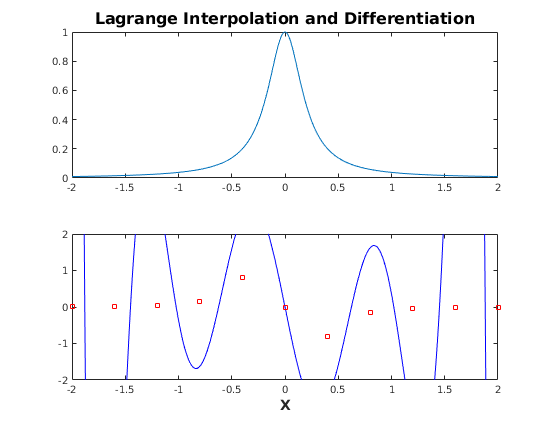
\includegraphics{lec18n-ex1-woa-n11-uniform.png}
\caption{Numeric differentiation with $n=11$ uniformly spaced points.}
\label{fig:lec18n-ex1-woa-n11-uniform}
\end{marginfigure}
Using $n=11$ uniformly spaced sample points, the function and its numerical derivative is shown in Figure \ref{fig:lec18n-ex1-woa-n11-uniform}.  The numerical derivative is of very poor quality. For uniformly spaced points, however, the quality does not improve if $n$ is increased.  The result for $n=21$ is shown in Figure \ref{fig:lec18n-ex1-woa-n21-uniform}. If anything, the numeric derivative is worse.
\begin{marginfigure}[-14.0cm]
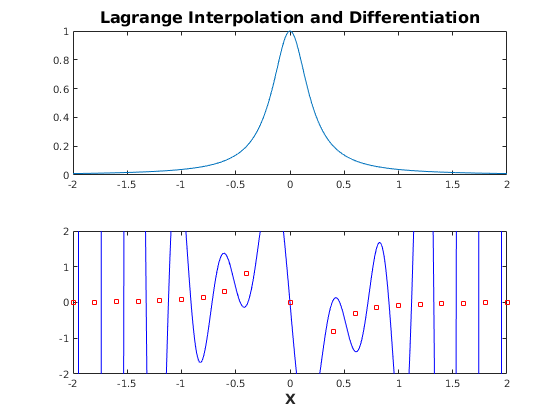
\includegraphics{lec18n-ex1-woa-n21-uniform.png}
\caption{Numeric differentiation with $n=21$ uniformly spaced points.}
\label{fig:lec18n-ex1-woa-n21-uniform}
\end{marginfigure}
\begin{marginfigure}[-4.0cm]
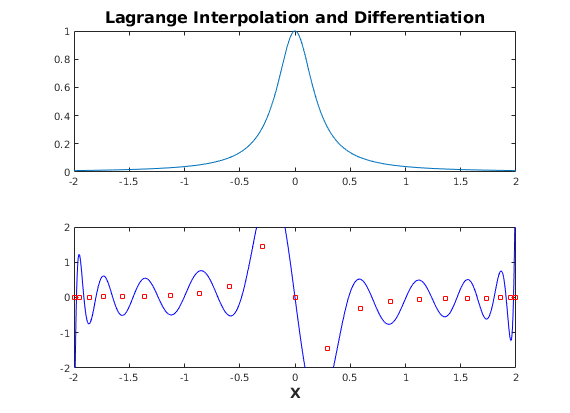
\includegraphics{lec18n-ex1-woa-n21-cheb.png}
\caption{Numeric differentiation with $n=21$ non-uniformly spaced points.}
\label{fig:lec18n-ex1-woa-n21-cheb}
\end{marginfigure}
In contrast, if we use non-uniformy spaced Chebychev points, as we did in Lecture 15, the quality of the numeric derivative is markedly better as we see in Figure \ref{fig:lec18n-ex1-woa-n21-cheb}.  Furthermore, if we increase the number of interpolation points, the quality of the numeric derivative improves still further as is shown in Figure \ref{fig:lec18n-ex1-woa-n51-cheb}.
\begin{marginfigure}[0.0cm]
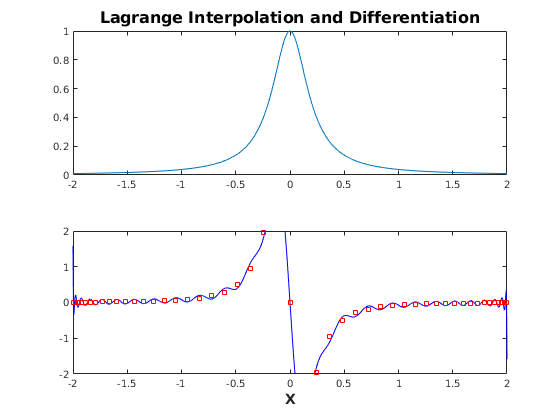
\includegraphics{lec18n-ex1-woa-n51-cheb.png}
\caption{Numeric differentiation with $n=51$ non-uniformly spaced points.}
\label{fig:lec18n-ex1-woa-n51-cheb}
\end{marginfigure}
When we study Finite Element Methods in future lectures, we will find numeric differentiation with Lagrange Polynomials using non-uniform sample points to be a very important and powerfull tool.

